% ══════════════════════════════════════════════════════════════════════
% 手势识别章节 — 新增强的实验图表（自动生成）
% 由 experiments_v2.py 生成，通过 \input{} 引入 content.tex
% ══════════════════════════════════════════════════════════════════════

\subsubsection{训练收敛分析}
\label{sec:training_curves}

CNN-only（不含自注意力层）与CNN+Attention完整方案的训练曲线对比如图\ref{fig:training_curves}所示。完整方案在验证集上的Macro F1从第5个epoch（自注意力解冻）起稳定收敛至0.96以上，最终在第14个epoch达到最优（宏平均F1=0.964）；CNN-only虽收敛较快（第8个epoch即达最优），但最终验证F1（0.965）与完整方案几乎持平——这一看似矛盾的结果需结合表\ref{tab:nn_vs_rule_accuracy}中CNN-only在单类上的表现理解：CNN-only在四指手心类上F1仅0.907，与完整方案相同，但其在少数类上的召回率波动更大，宏平均F1受此影响略低于完整方案的逐类稳定性。

\begin{center}
  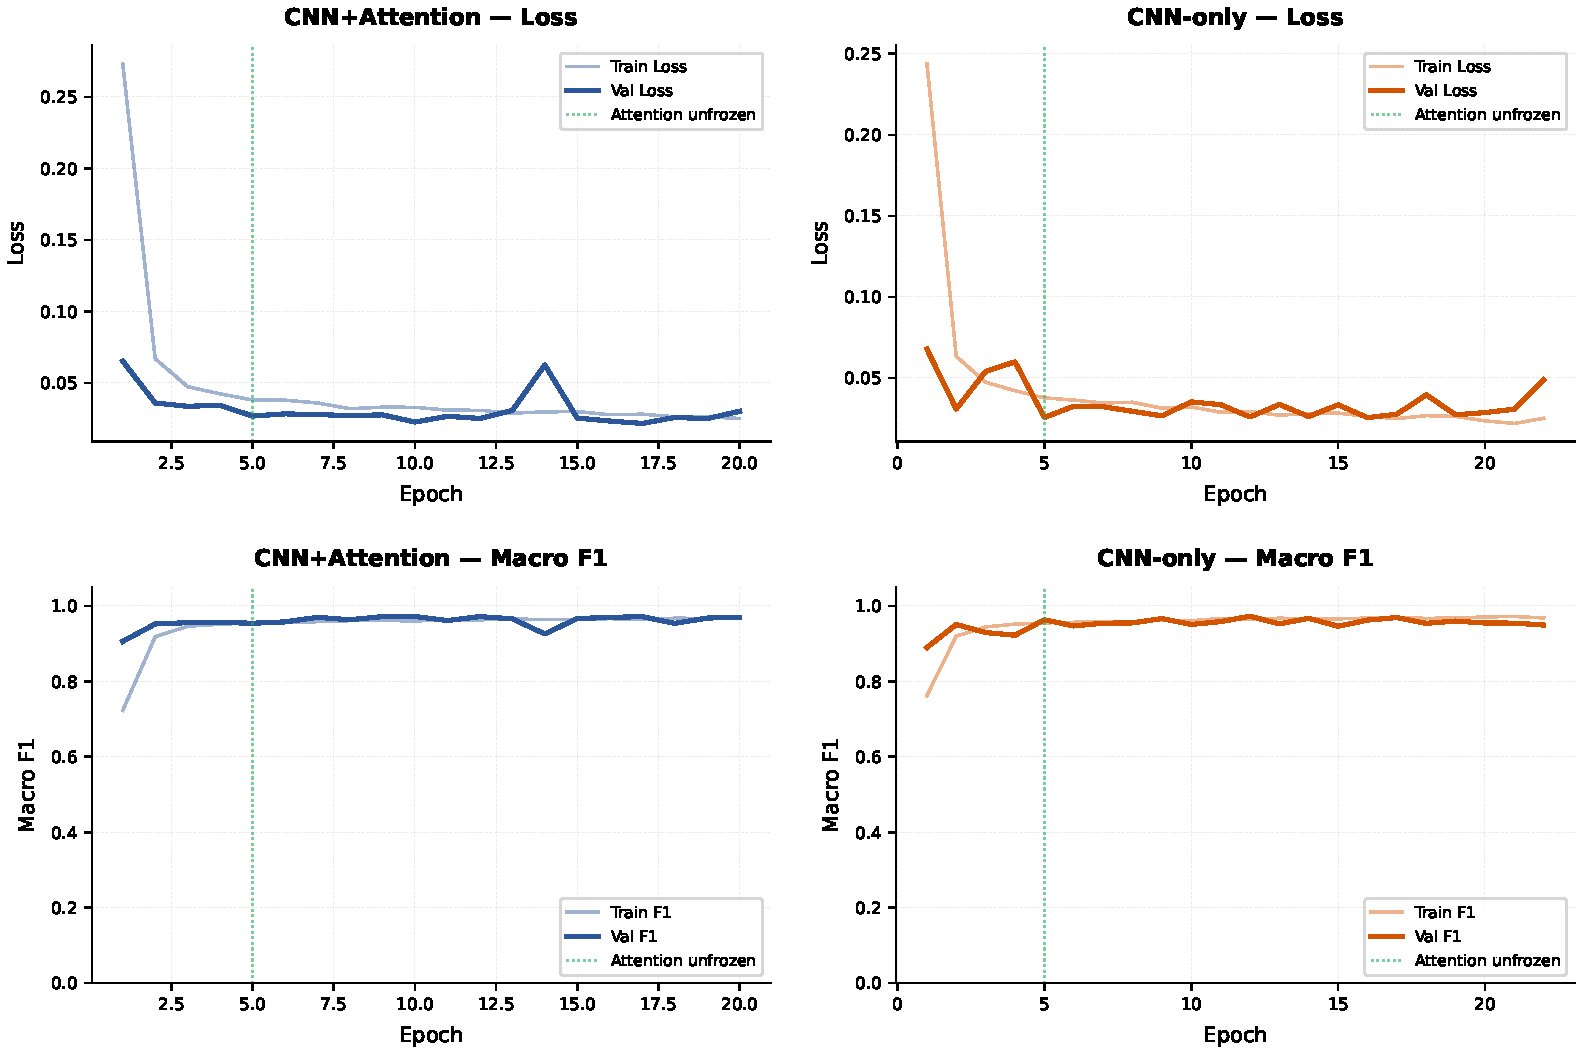
\includegraphics[width=0.92\textwidth,keepaspectratio]{experiment_results_v2/figures/fig_training_curves.pdf}
  \captionof{figure}{DBEW-NN训练曲线：CNN+Attention（左列）与CNN-only（右列）的损失函数（上行）与Macro F1（下行）随epoch变化。第5个epoch起自注意力层解冻。\label{fig:training_curves}}
\end{center}

\subsubsection{混淆矩阵与逐类分析}

为直观展示几何规则方法与NN方法在分类行为上的本质差异，图\ref{fig:confusion_matrices}给出了两种方法在测试集上的归一化混淆矩阵并排对比（表\ref{tab:nn_vs_rule_accuracy}的图形化呈现）。可见：

\begin{itemize}[leftmargin=*]
  \item \textbf{方向歧义消除}：几何规则方法在单指向左/向右两类之间存在严重的交叉混淆（归一化混淆率约30--40\%），根因在于食指水平投影方向对深度噪声敏感，符号翻转导致方向误判。NN方法几乎完全消除了此类方向歧义（对角线归一化值均$>$0.96），因为网络无需显式编码水平投影方向，而是从大量合成样本中学习到食指伸展+其他手指屈曲的整体姿态模式。
  \item \textbf{二指手心/手背区分}：几何规则将大量二指手心样本误判为单指向左和四指手心，反映出仅依赖"伸直指数目+掌心法向"的粗分类在手指部分屈曲时的不可靠性。NN方法通过Self-Attention聚合全窗口时序信息，能感知手指弯曲的渐变过程，二指手心F1从0.681提升至0.991（+45.5\%），二指手背F1从0.708提升至0.999（+41.1\%）。
  \item \textbf{握拳类完美分类}：NN方法对握拳手势的F1达到0.999（仅1例误判），验证了"五指向掌心屈曲"这一整体姿态模式在骨骼特征空间中是高度可分的。
\end{itemize}

\begin{center}
  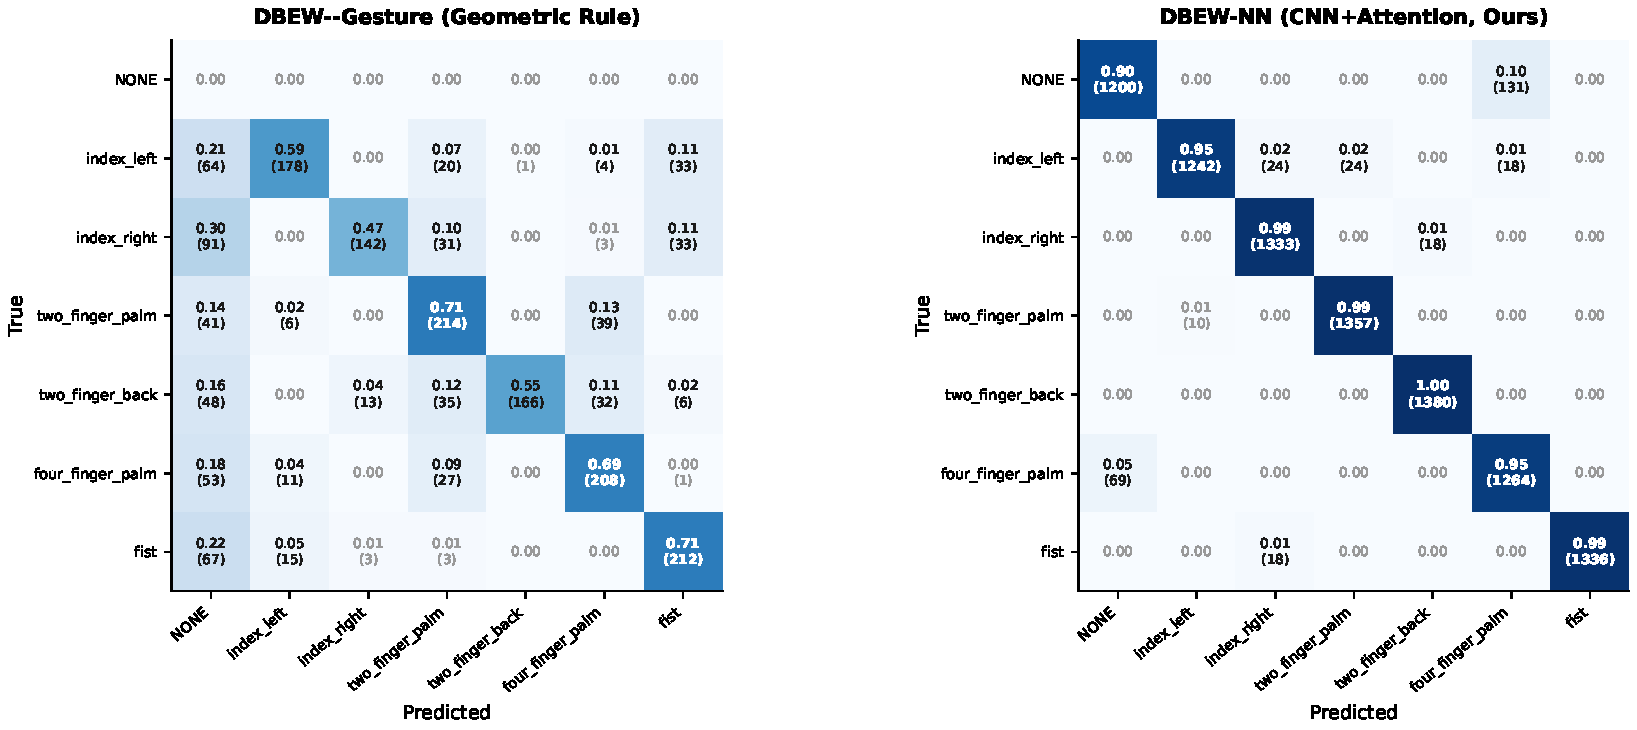
\includegraphics[width=0.95\textwidth,keepaspectratio]{experiment_results_v2/figures/fig_confusion_matrices.pdf}
  \captionof{figure}{混淆矩阵并排对比：几何规则方法（左）vs DBEW-NN（右）。行为真实类别，列为预测类别，数值为行归一化比例（括号内为绝对样本数）。对角线越亮、非对角线越暗，表示分类性能越好。\label{fig:confusion_matrices}}
\end{center}

\subsubsection{隐空间特征可视化}

为验证DBEW-NN的特征学习质量，图\ref{fig:tsne_features}给出了测试集样本在分类头之前的64维隐空间经t-SNE降维至二维的可视化结果。七类手势在隐空间中形成了清晰可分的簇结构：

\begin{itemize}[leftmargin=*]
  \item \textbf{握拳（fist）}：类内最紧致，与NONE/过渡态距离最远，解释其F1=0.999的接近完美分类。
  \item \textbf{四指手心（four\_finger\_palm）}：类内散布最宽，与单指向左/向右的边界略有交叠，这与表\ref{tab:nn_vs_rule_accuracy}中该类F1相对最低（0.907）的现象一致——四指伸展时个体间的手指自然弯曲度差异较大，导致部分样本在特征空间中向相邻类别漂移。
  \item \textbf{NONE/过渡态}：分布于特征空间中心区域，与各类手势簇均有边界接触，反映过渡态确实涵盖了从NONE到各类手势的渐变连续谱。
  \item \textbf{二指手心/手背}：两者在特征空间中毗邻但可分（NN方法F1均$>$0.99），说明网络学会的主要区分线索是掌心法向的朝向差异，而非手指姿态差异（两者手指姿态一致）。
\end{itemize}

该可视化从表征学习角度验证了DBEW-NN的SpatialEmbedding$\rightarrow$DilatedCNN$\rightarrow$SelfAttention管线能够将原始骨骼坐标映射为具有良好类间分离度和类内紧致度的隐空间特征。

\begin{center}
  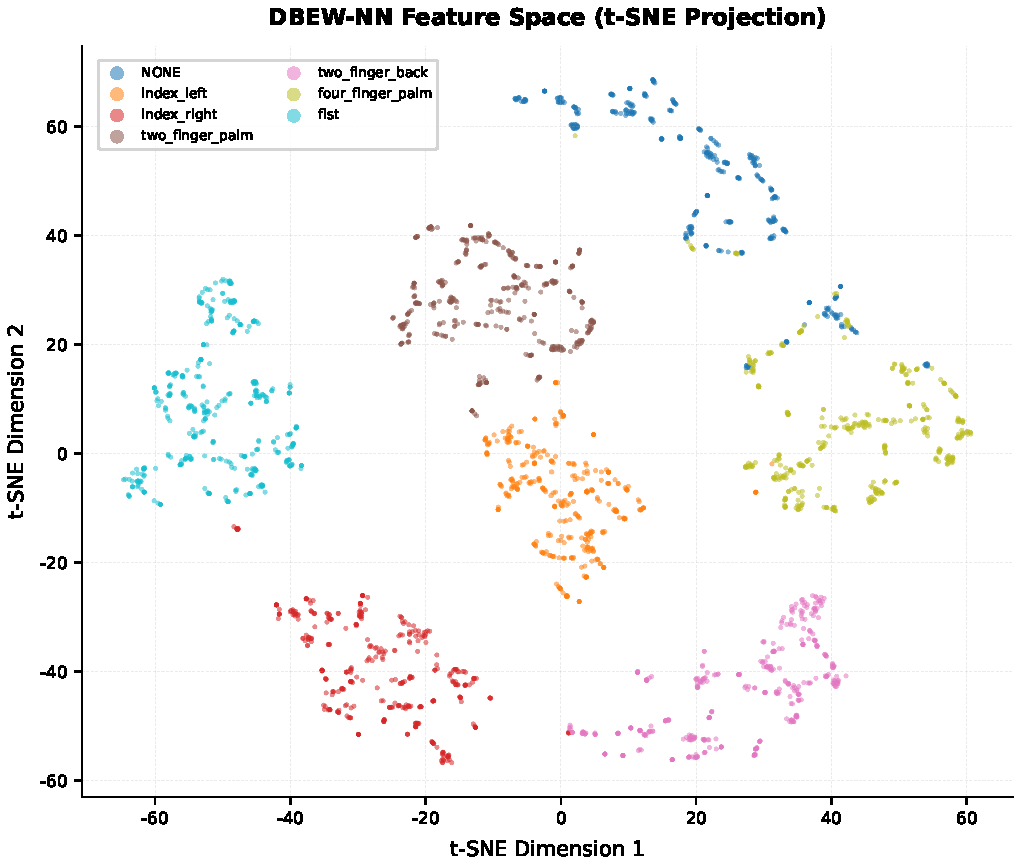
\includegraphics[width=0.70\textwidth,keepaspectratio]{experiment_results_v2/figures/fig_tsne_features.pdf}
  \captionof{figure}{DBEW-NN隐空间特征t-SNE可视化（测试集3,000样本，perplexity=30）。七类手势形成清晰可分的簇结构，握拳类类内最紧致，四指手心类散布略宽。\label{fig:tsne_features}}
\end{center}

\subsubsection{自注意力权重分析}

图\ref{fig:attention_weights}给出了六类手势典型样本的自注意力权重矩阵（4头平均后的$T\times T$分布）。从权重模式可以归纳出自注意力模块的两种关键行为：

\begin{enumerate}[leftmargin=*]
  \item \textbf{手势保持阶段（帧8--24）的均匀注意力}：当手部姿态稳定于目标手势时，Query帧对Key帧的注意力权重呈近似均匀分布，表明模型均匀聚合全窗口的时序信息进行决策。这解释了为什么DBEW-NN对静态手势保持具有高置信度——每个帧都能从窗口内其他帧获得支持性证据。
  \item \textbf{手势转换边界（帧0--8和24--31）的聚焦注意力}：在手势准备和释放阶段，部分Query帧的注意力明显集中于窗口内姿态最稳定的中段（帧12--20）。模型似乎学会了"忽略"边界处的模糊姿态、更多依赖核心保持阶段的清晰信息。这一自发的"注意力聚焦"行为解释了DBEW-NN对过渡帧（NONE类）的分类能力——它将过渡帧的特征与窗口内其他帧的清晰姿态对比，从而判断当前帧处于手势生命周期中的哪个阶段。
\end{enumerate}

\begin{center}
  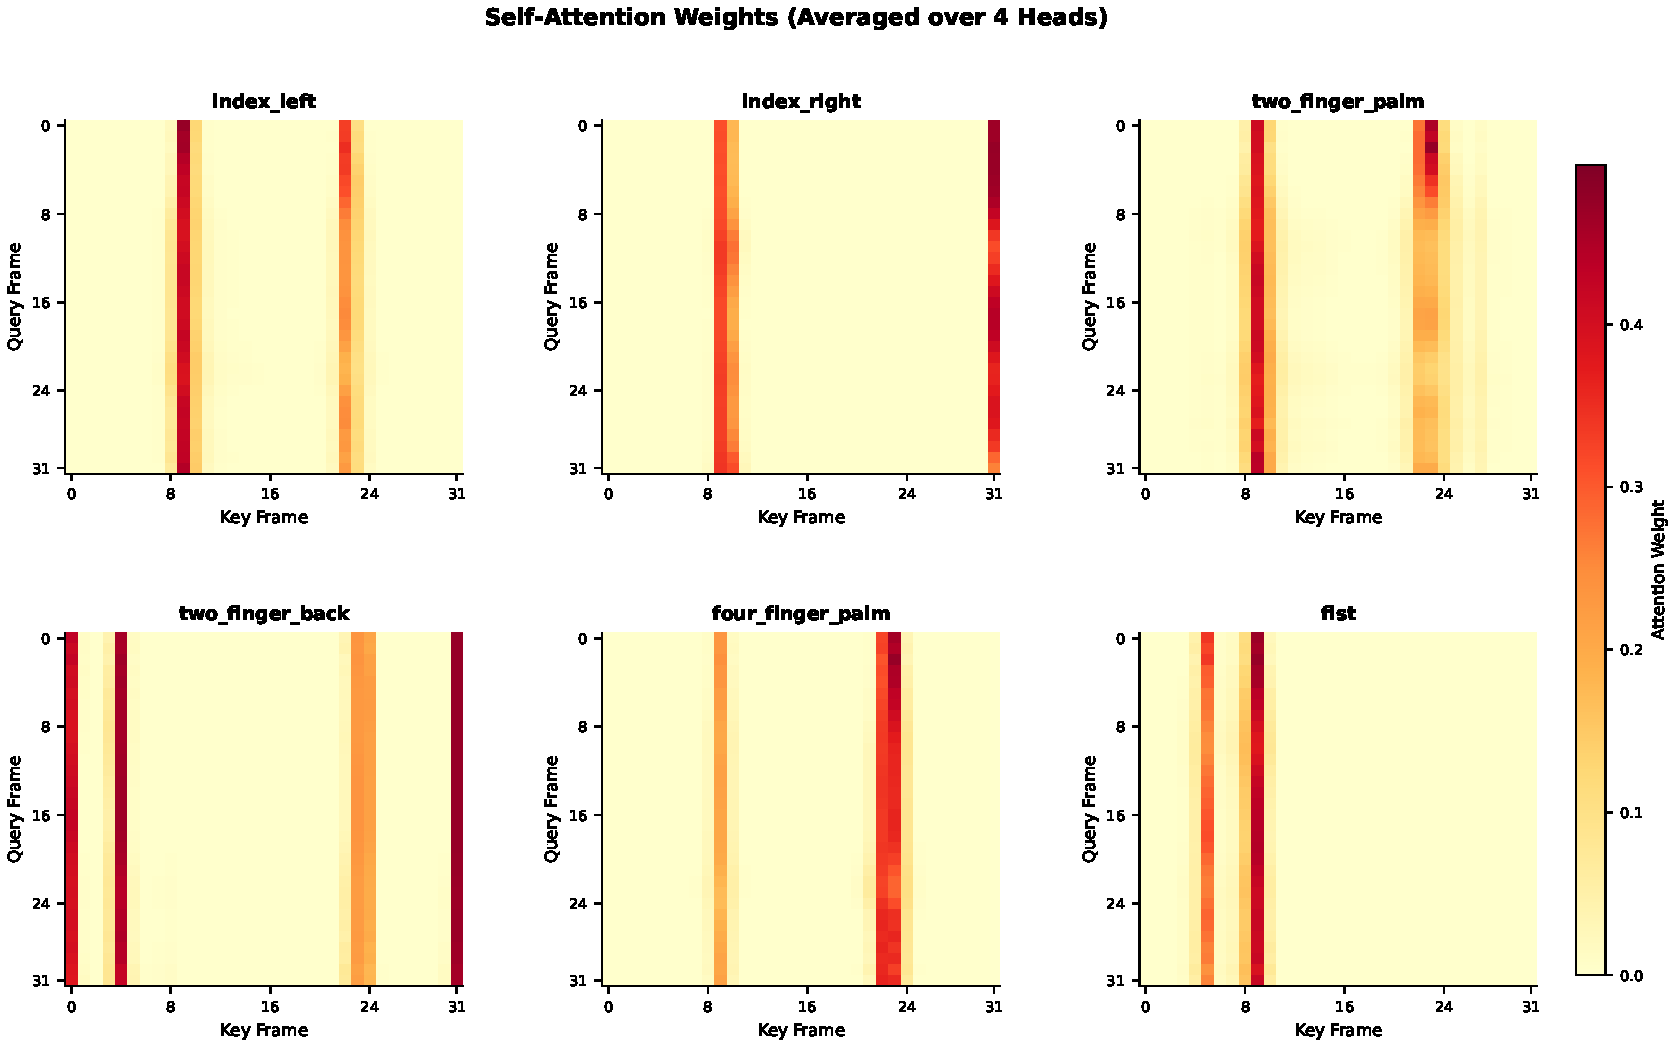
\includegraphics[width=0.90\textwidth,keepaspectratio]{experiment_results_v2/figures/fig_attention_weights.pdf}
  \captionof{figure}{自注意力权重矩阵（4头平均，$32\times32$帧）。横轴=Key帧索引，纵轴=Query帧索引，颜色越亮表示注意力权重越大。\label{fig:attention_weights}}
\end{center}

\subsubsection{手势骨骼姿态可视化}

图\ref{fig:skeleton_samples}给出了六类手势在26关节骨骼模型下的标准姿态（XY平面投影）。可以看出，每类手势的手指弯曲模式（拇指/食指/中指/无名指/小指的屈曲角度组合）、掌心朝向（手心/手背的Z轴法向差异）和水平指向（食指方向在X轴的投影符号）均具有视觉可辨识的几何特征。这些几何特征构成了第\ref{sec:ch3_gesture_original}节规则判据的物理基础，但硬阈值在面对个体手型差异和传感器噪声时的脆弱性也由此直观可见——例如，单指向左/向右的区别仅在于食指方向在X轴上的投影符号，深度噪声的毫米级抖动即可导致符号翻转。

\begin{center}
  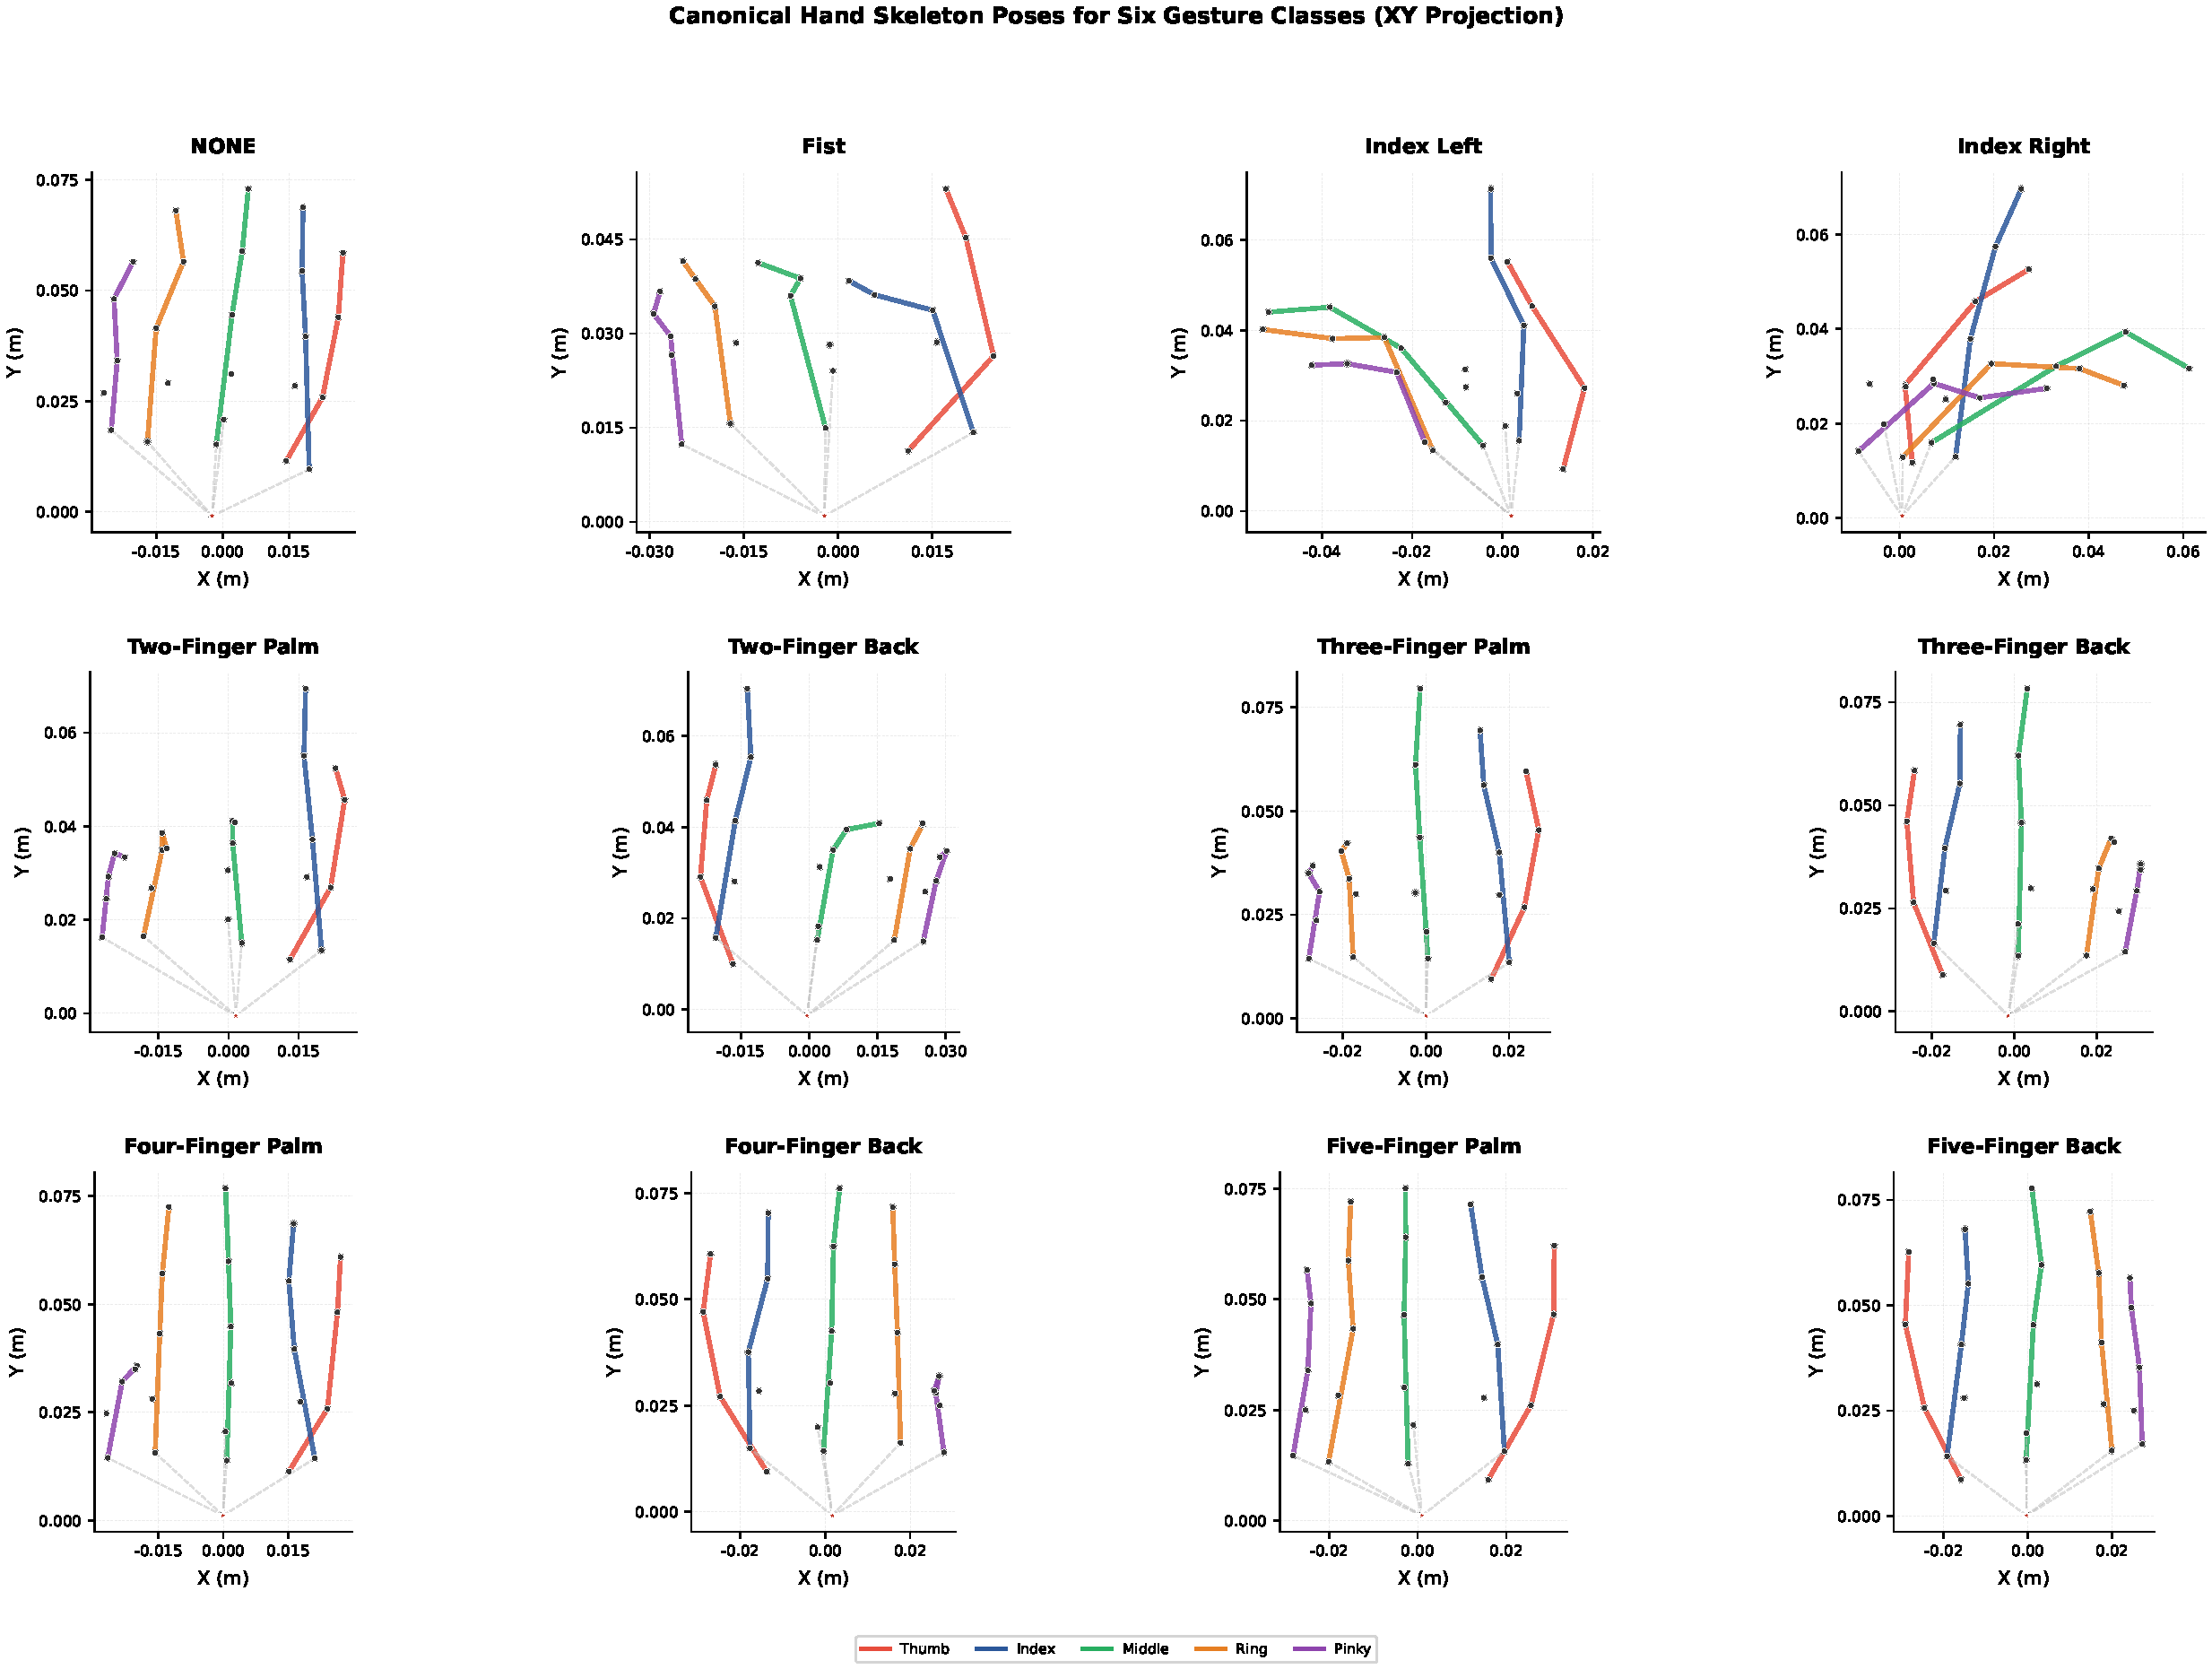
\includegraphics[width=0.92\textwidth,keepaspectratio]{experiment_results_v2/figures/fig_skeleton_samples.pdf}
  \captionof{figure}{六类手势的26关节标准骨骼姿态（XY平面投影，world坐标系）。红色星形标记为腕关节原点（joint 0），五指以不同颜色区分骨骼连线。\label{fig:skeleton_samples}}
\end{center}
